%%%%%%%%%%%%%%%%%%%%%%% file moduleX_template.tex %%%%%%%%%%%%%%%%%
%
%
% This is a template for creating your papers for the course KRW
% It is based on the standard Latex template for Springer publications
% but contains a suggestion for the structure and some content of the
% paper.
%
% Please adapt this document wherever needed.
%
% For more information about the required Latex Style check the document
% typeinst.pdf in the StyleFiles directory.
%
%%%%%%%%%%%%%%%%%%%%%%%%%%%%%%%%%%%%%%%%%%%%%%%%%%%%%%%%%%%%%%%%%%%%%%%%%


\documentclass[runningheads,a4paper]{../../StyleFiles/llncs}

\usepackage{url}
\usepackage{graphicx}
\usepackage{amssymb}
\usepackage{listings}


\newcommand{\keywords}[1]{\par\addvspace\baselineskip
\noindent\keywordname\enspace\ignorespaces#1}

\begin{document}

\mainmatter  % start of an individual contribution

% first the title is needed
\title{Data- and Ontology Paper: Quality Ontology for Handicap Parking Spots around Venues in Amsterdam}

% a short form should be given in case it is too long for the running head
\titlerunning{Data- and Ontology Paper}

% the name(s) of the author(s) follow(s) next
%
% NB: Chinese authors should write their first names(s) in front of
% their surnames. This ensures that the names appear correctly in
% the running heads and the author index.
%
\author{Alivanistos, Dimitris. \\ Baez, Selene. \\ Jemmett, Andrea. }
%
\authorrunning{Alivanistos, Dimitris. \\ Baez, Selene. \\ Jemmett, Andrea.}
% (feature abused for this document to repeat the title also on left hand pages)

% the affiliations are given next; don't give your e-mail address
% unless you accept that it will be published
\institute{\url{d.alivanistos@student.vu.nl} \and \url{s.baezsantamaria@student.vu.nl} \and \url{a.jemmett@student.vu.nl}}

\maketitle


\begin{abstract}
The abstract should summarize the contents of the paper and should
contain at least 70 and at most 150 words. It should be written using the
\emph{abstract} environment.
\end{abstract}


\section{Section 1 - Introduction}
\textit{Introduce the sections that follow. What is the core contribution of this paper, and why is that interesting? It is useful to start with a use case (practical/theoretical), and then explain how your ontology (will) solve(s) that problem by means of KR technology. Why is this novel? Has this (or something similar) been done before?}

- Information about handicap parking spots in Amsterdam is not well organized. Datasets exists and are available to the public but they are not well structures in a human readable manner. 

- We focus on a particular usage of such parking spots, those linked to events happening in the city of Amsterdam. 

- Our ontology organizes the events and venues into subtypes. This brings clarity for users who have special interest. (E.g. Toribio is only interested in theater plays. He is in a wheelchair and needs accessible parking spots to go to Theaters when he selects a play to watch).

- Our ontology has organized knowledge about addresses. It treats Streets and Postal codes as entities. Thus, a postal code is related to a set of events, a set of venues, and a set of parking spots. (E.g. Chachita has appointments once every week at the Femme Amsterdam Hospital. She would like to look for events nearby to attend after her sessions.)
(NOTE: important entailment here!!!! if we know a venue is in a postal code, all events related to the venue must be related to the same postal code.)

%TODO: is this novel? Website for accesible amsterdam does not have anything similar. 

\section{Section 2 - Use Case and Requirements}
\textit{Describe the use-case you have in mind that motivates the need for the ontology. This could be the original use case from milestone 1, but then you should explain why the schema you defined previously falls short. What requirements should the ontology meet? What is its intended scope.}
\subsection{Previous use cases}
\begin{enumerate}
	% Planning in advance
	\item John is in a wheelchair and wants to go to an exhibition in Van Gogh Museum Friday night. John likes to plan things in advance and would like to know where the parking slots closest to the theater are. \\
	The day before the show, John uses our application to find such parking slots and heads to the show confidently. 
	% Quick search once in the theater (on the fly)
	\item Peter broke his leg last month and his friends, as an attempt to cheer him up, invited him to come to a comedy show at the Comedy Cafe. He is quite late and he is rushing to find the closest parking slots. He quickly browses our application and finds an area with several parking slots. He drives in that direction hoping to find an available slot. 
	% Event manager
	\item Mary is an event organizer who wants to host an exhibition in a museum next month. She is looking for an accessible venue so she would like to see the distribution of parking slots around the main galleries in Amsterdam. She has a list of five places in mind and uses our application to explore and choose the best venue.
\end{enumerate}

\textbf{Why the previous schema falls short?}

- John and Peter have to go through a long list of events till they find the exhibition or show they are attending. A new ontology that subdivides events into types helps him navigate the data more easily. 

New use cases explained in the introduction. 

\subsection{Requiremnts}

\begin{enumerate}
	\item Search subset of events
	\item Detailed location information
	\item Detailed information about Parking Slots
\end{enumerate}


\section{Section 3 - Related Work}
\textit{What other ontologies did you find that cover a similar domain. To what extent can they be reused. Have others (e.g. other students) developed similar datasets/ontologies that feed/meet your requirements, where do they fall short? Papers to look for are published at eg. ISWC, ESWC, EKAW and FOIS, or the Journal of Web Semantics, and the Semantic Web Journal.}

 - Ontology for smart cities: \cite{komninos2015smart}


\section{Section 4 - Methodology}
\textit{Describe the methodology you followed for constructing the ontology. How did you guarantee that the ontology meets the needs and requirements of the use case? Have you used any existing design patterns, partial ontologies, competency questions etc.}

- Use of Protégé

- Iterative process.

- Subclasses, cardinality, object Properties

- Extensive use of powerful ontologies like dbo. Use of equivalence between dbo:Place and dbo:Location

\section{Section 5 - The Ontology}
\textit{Systematically describe the ontology and highlight the (interesting) design choices you had to make. Were there things you wanted to represent but couldn't given the limitations on the KR language?\footnote{If you do not encounter any limitations, you should be more ambitious about the model!} How did you work around these limitations? (integrity constraints, additional rules?) Describe how the ontology meets the 5 star model for Linked Vocabulary Use.}

%TODO insert image
\begin{figure}[h]
	\centering
	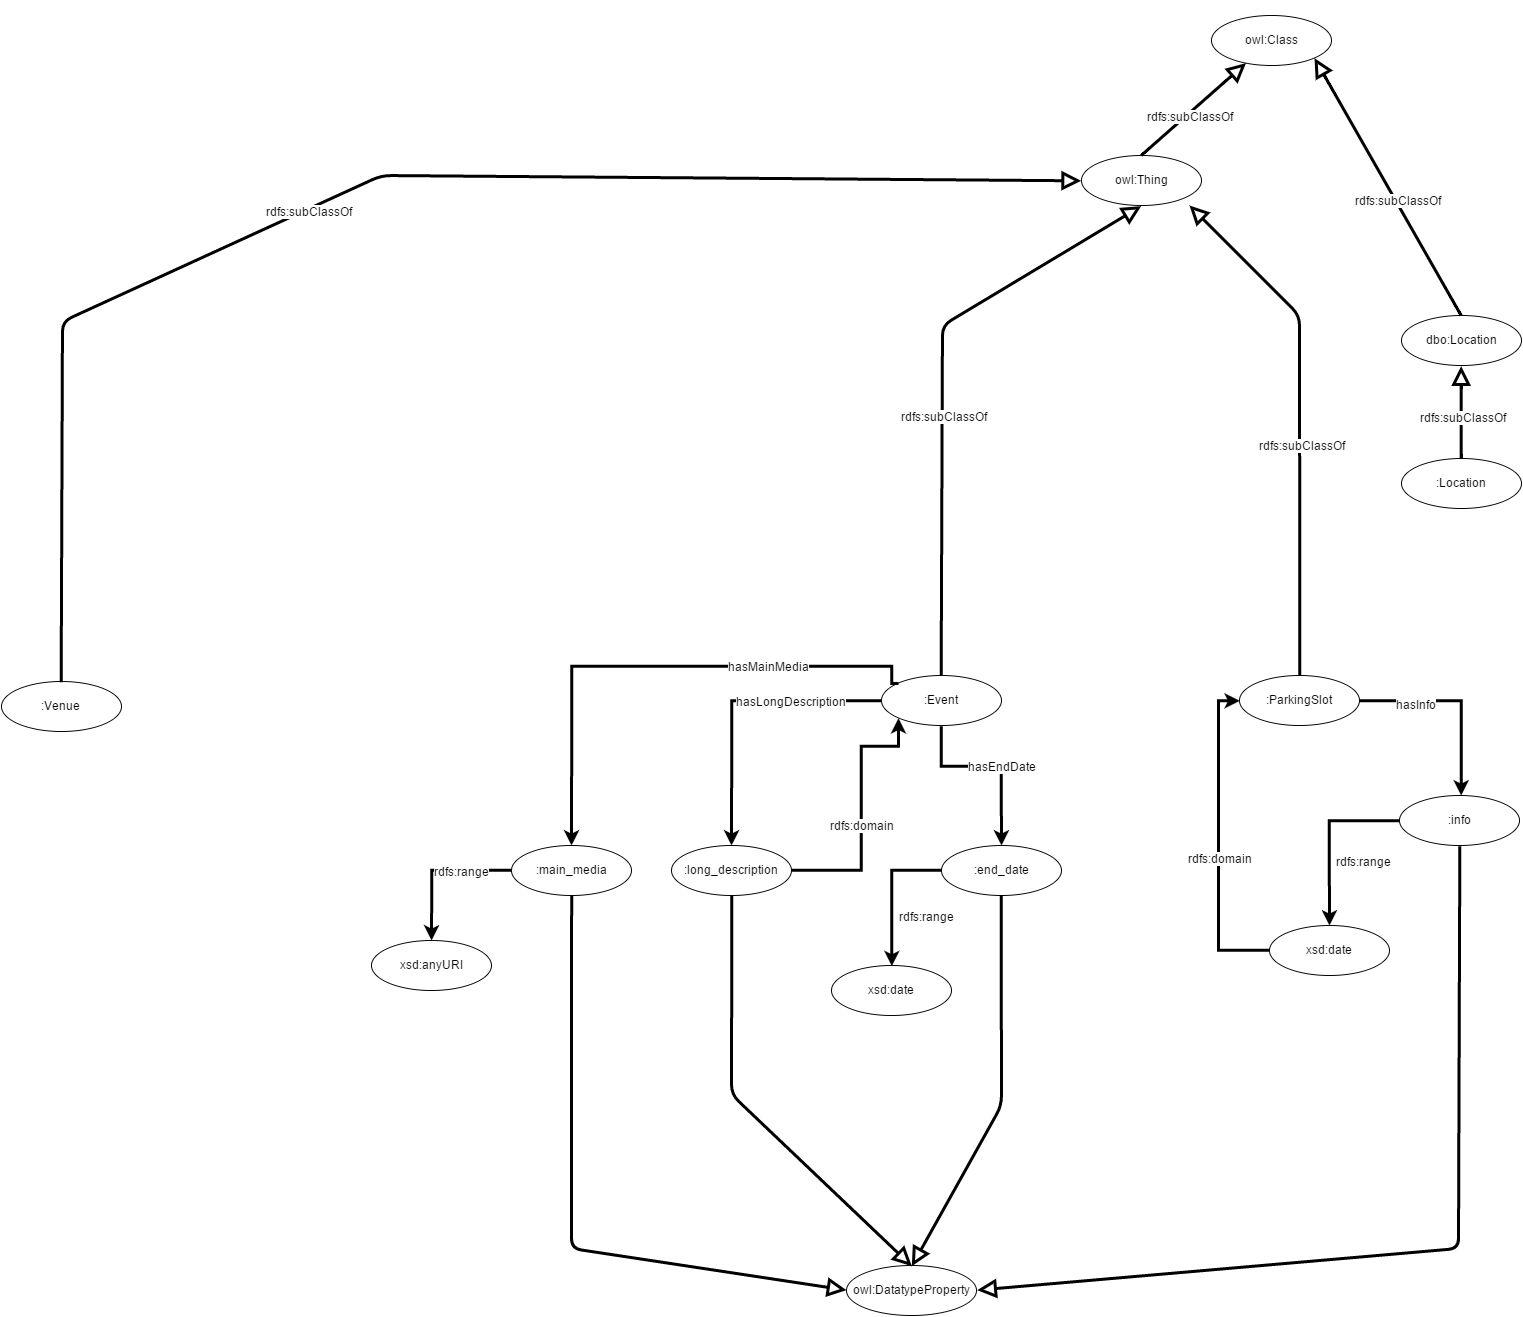
\includegraphics[width=.7\textwidth]{img/ontology.png}
	\caption{Visualization of the Ontology graph}
	\label{fig:ontology}
\end{figure}

\subsection{Entities}
- Now we have subclasses for each of the main type of classes we had before

- Events: into Plays and Exhibitions
- Venues into Theatres and Museums
- Parking Slot into Small Medium and Large

- First two distinctions come from the datasets themselves. The third one we created based on size. Parking Slot has datatype property quantity, which serves a a classifier

\begin{lstlisting}[captionpos=b, caption=Definition of Large Slot a subclass of Parking Slot, label=lst:sparql, basicstyle=\ttfamily\small,frame=bt]
(dbo:location exactly 1 Location)
and (info exactly 1 xsd:string)
and (quantity exactly 1 xsd:unsignedInt)
\end{lstlisting}

- Our Location class extends dbo:Location class in the use of Borough

\subsection{Properties}

- Restrictions on datatype properties. Cardinalities are explicit, so that they reflect that an Event has only one Venue, for example

- Introduce 'Event venue' which has subproperties 'Exhibition Venue' and 'Play Venue' depending on their range. Also introduce its inverse 'Venue Events'

- We create a subproperty of dbo:location to be 'venue location'. We restrict dbo:location to have domain Parking Slots while 'venue location' has domain Venues. Both have Location as range.

- Properties for Borough, City and Country


\section{Section 6 - The Dataset}
Describe how you recasted the dataset(s) of the previous assignment to the new ontology (perhaps you found other datasets that you want to add). What did it take to do this? What metadata have you published alongside the dataset, and how did you generate it? (Provenance, VOID, etc.) Describe how your data meeds the 5 star model for Linked Data.

\section{Section 7 - Evaluation}
Evaluate the ontology and dataset with respect to each other (does the ontology really sanction only the intended inference) and with respect to the requirements and use case (extend your application?!). You may want to analyze the ontology using some quality criteria from the literature.

\section{Discussion}
Here you summarize the preceding sections, describe the lessons learnt and discuss future work.


\bibliographystyle{plain}
\bibliography{mybib}

\end{document}
